%%%%%%%%%%%%%%%%%%%%%%%%%%%%%%%%%%%%%
%%%%% PHYS305 Assignment 2
%%%%% Zachary Martin
%%%%% 28 January 2019
%%%%%%%%%%%%%%%%%%%%%%%%%%%%%%%%%%%%%

\documentclass[aps,prl,twocolumn,superscriptaddress]{revtex4-1}

\usepackage{graphicx}  % this is the up-to-date package for all figures
\graphicspath{{pictures/}} 	% Set Graphics Path
\usepackage{siunitx} % Scientific Notation and Units
\usepackage{amsmath, amssymb, gensymb, mathtools, bm} 	% Mathematical Tools
\usepackage{verbatim}  % for the comment environment
\usepackage{color}
% \usepackage{arydshln} % Dashed lines in table

% For inserting code snippets
\usepackage{listings}
\usepackage{xcolor}
\lstset { %
    language=C++,
    backgroundcolor=\color{black!5}, % set backgroundcolor
    basicstyle=\footnotesize,% basic font setting
}

% Shortcut Commands
\newcommand{\paren}[1]{\left( #1 \right)} 	% Parentheses for complicated expressions
\newcommand{\bparen}[1]{\left[ #1 \right]}	% Bracket parentheses for complicated expressions
\newcommand{\cmod}[1]{\left| #1 \right|}	% Mod or Absolute value

\bibliographystyle{apsrev}

% these are some custom control of the page size and margins
% \topmargin= 0.2in  % these 1st two may be needed for some computers
\textheight=9in
\textwidth=6.5in
% these next two lines give us centered text
\oddsidemargin=0cm
\evensidemargin=0cm

\begin{document}

% Title Contents
\title{PHYS 305 Assignment 2: Analyzing the Behavior of a Bouncing Ball with Energy Loss per Bounce and Machine Precision.}
\author{Zachary Martin}
\affiliation{University of Hawaii at Manoa}
\date{30 January 2019}

\begin{abstract}
In this assignment, we examine the behavior of a bouncing ball whose energy changes according to a coefficient of restoration, $C$, for each bounce. We will write a program using C++ to calculate the bounce heights and times, and the accumulation of those to get the total distance and total time for a given number of bounces. We find just what we would expect, that the total reaches a positive limit as the terms decrease to 0. We also find that the time it takes for the ball's bounce height to reach 0 increases exponentially towards infinity as $C$ increases towards 1. We will also use this experiment to examine the precision of the computer using float vs double type values, and find that floats give an accuracy only to the 6th or 7th digit.
\end{abstract}

\maketitle

\section{Introduction and Overview}
Many systems we encounter in physics are not conservative in reality. There are usually energy losses as the system evolves in time. It is therefore important to be able to analyze these systems where the total energy is lost due to non-conservative forces. We will consider systems whose energies can be described as some factor of the initial energy. One such case is a bouncing ball whose energy will change by some coefficient of restoration $C$ for each bounce. 

When doing calculations using a computer, it is important to realize how the computer stores these numbers. When writing a program in C++, we can have float-type values which have single precision (32 bit) or double-type values which have double precision (64 bit) \cite{Laulima}. In general, it is advantageous to use floating points over double points as the computer can perform more quickly with floating points, however we lose some accuracy. We need to know how far the accuracy goes in terms of digits so that we can recognize when we can use float-type values in our calculations or when we need to use double-type values.

\section{Description of Computational Problem}
We want both the calculations of each term, height and time, per bounce as well as the total distance and time. To do this, we must split the problem up into parts based on the bounce cycle. We can consider one cycle and calculate those terms starting from $E = E_0$. Then we can apply the next energy, $E_1 = C E_0$, and find the terms for that new energy. We can continue to do this for $N_{\text{max}}$ terms and finally accumulate them in a summation.

To examine the machine precision, we will do this calculation twice, first using float-type values and then again using double-type values. We can then directly compare the values we get for the data and determine the digits of accuracy for floats.

\section{Relevant Equations}
We begin by considering a bouncing ball whose energy changes by a factor of some coefficient of restoration per bounce, that is,
\begin{equation}
	E_n = C^n E_0 ~.
\end{equation}
We assume that the ball has mass $m = \SI{1.0}{\kg}$ and begins at a height $h = \SI{1.0}{\m}$. In order to analyze the changing energy's effect on the bounce height and time, it is necessary to consider the equations for conservation of energy. To calculate the time, we first need the initial speed immediately after bouncing. This comes from taking the total energy to be the kinetic energy, that is,
\begin{align}
	E &= \frac{1}{2}mv^2 \\
	\Rightarrow ~ v &= \sqrt{\frac{2E}{m}} ~.
\end{align}
Then using kinematic equations with acceleration equal to gravity, we find
\begin{align}
	v &= v_0 + at \\
	\Rightarrow ~ t &= \frac{1}{g} \sqrt{\frac{2E}{m}} ~.
\end{align}
For the bounce height, the total energy at the top is just the potential energy due to gravity, and so
\begin{align}
	E &= mgy \\
	\Rightarrow ~ y &= \frac{E}{mg} ~.
\end{align}
Inputting our results into the program yields the functions
\begin{lstlisting}
float tbounce(float Eb) 
{
    float t =  pow(2*Eb/m, 0.5)/g;
    return(t);
}

float ybounce(float Eb)
{
    float y = Eb/(m*g);
    return (y);
\end{lstlisting}
We can go through half a bounce starting with the ball at the height $\SI{1.0}{\m}$. Then to accumulate the results of each bounce thereafter, we use the script
\begin{lstlisting}
for(int k=0;k< Nmax;k++){
    tterm = tbounce(E);
    tsum += 2.*tterm; 
// up then down gives factor of 2
    yterm = ybounce(E);
    ysum += 2.*yterm;
    n += 2;  
// add two half-bounces to the total
    E *= C;
\end{lstlisting}

\section{Results and Graphs}

Our results are summarized in Figures \ref{gr:gen} - \ref{gr:HvT} and discussed in the next section.

\begin{figure}[htbp]
 	\begin{center}
 		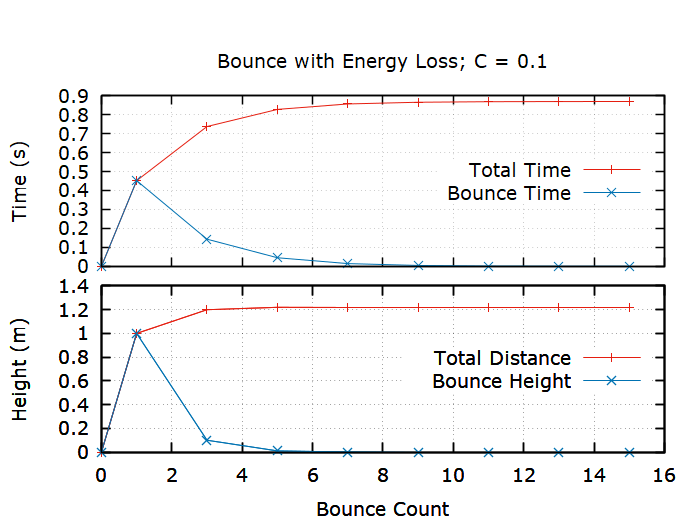
\includegraphics[scale=0.27]{01.png}
  		
 		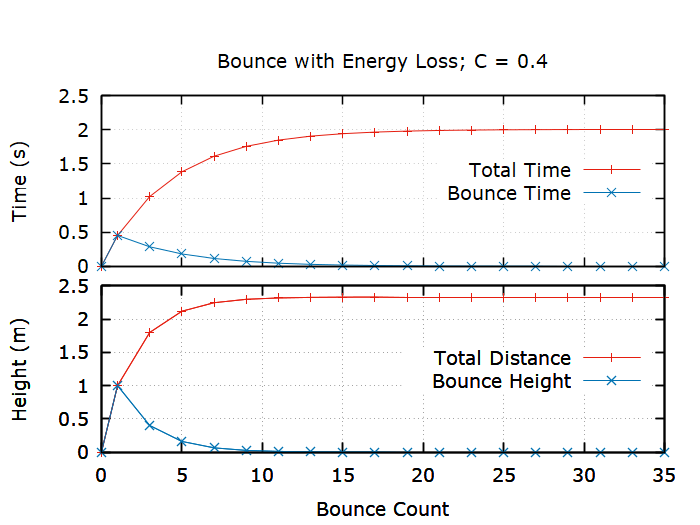
\includegraphics[scale=0.27]{04.png}
  		
 		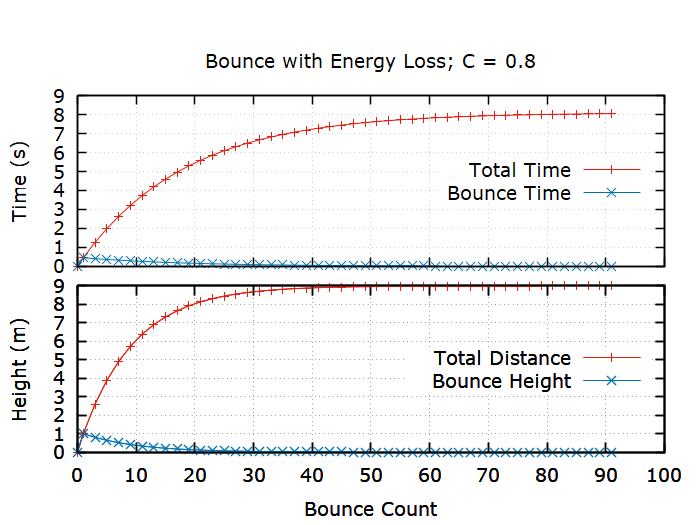
\includegraphics[scale=0.27]{08.png} 
  		\caption{A look at how the $n^{\text{th}}$ bounce time and height, as well as the total time and height, change throughout the bounces. Note how the total plateaus to a positive value as the bounce term approaches 0. It is easy to see from these graphs that the function of the bounce terms with respect to the bounces describes the derivative of the function of the total terms with respect to the bounces.}
  		\label{gr:gen}
 	\end{center}
\end{figure}

\begin{figure}[htbp]
 	\begin{center}
 		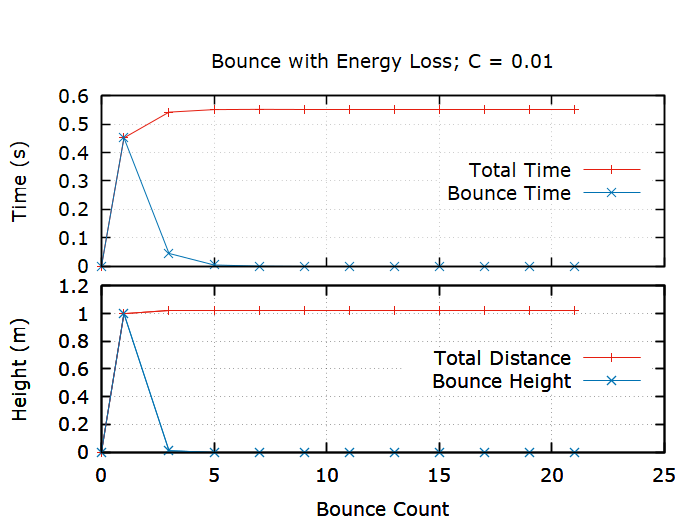
\includegraphics[scale=0.27]{001.png} 
  		\caption{Lower limit extreme of the coefficient of restoration. The values reach a constant very quickly, that is, the ball hits the ground and doesn't come back up. Note that the computer could not distinguish differences in the value at higher $n$, despite the mathematical fact that the ball never does exactly reach a constant total distance or total time (bounce height and time never exactly 0 mathematically).}
  		\label{gr:0.01}
 	\end{center}
\end{figure}

\begin{figure}[htbp]
 	\begin{center}
 		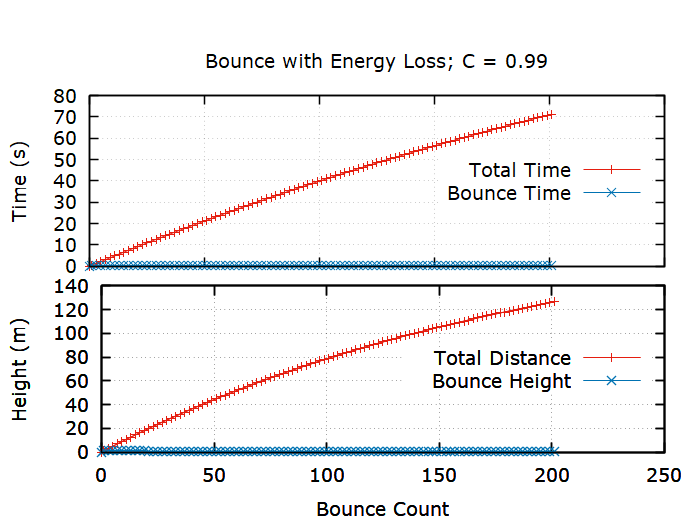
\includegraphics[scale=0.27]{099.png} 
  		\caption{Upper limit extreme of the coefficient of restoration. The values dampen very weakly through each bounce. Each bounce height is below $\SI{1.0}{\m}$ but 99\% of that height is retained in the next bounce, resulting in a total distance much greater than $\SI{1.0}{\m}$.}
  		\label{gr:0.99}
 	\end{center}
\end{figure}

\begin{figure}[htbp]
 	\begin{center}
 		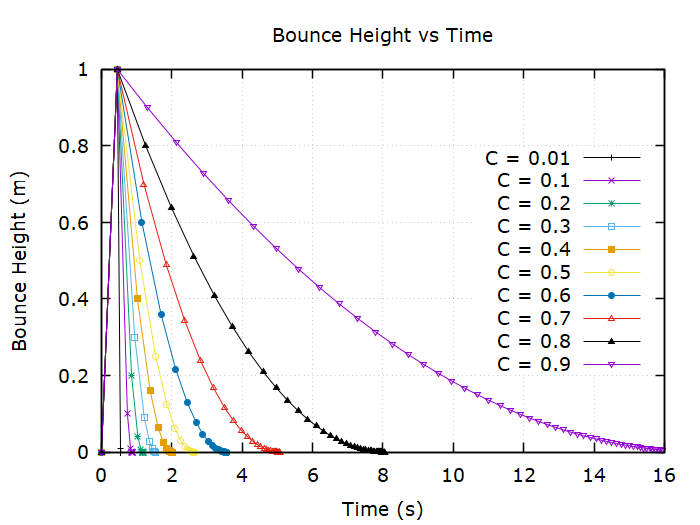
\includegraphics[scale=0.3]{HvT.png} 
  		\caption{A plot of the bounce height as a function of time for different coefficients of restoration. Note that the curve for $C = 0.99$ would reach much much greater than $\SI{16}{\s}$ and dominate the other curves, thus it is not graphed here.}
  		\label{gr:HvT}
 	\end{center}
\end{figure}

\section{Discussion and Analysis}

\subsection{The Bouncing Ball}
We were able to collect the values of the bounce terms and the total distance and time throughout the bounces using the script in the Relevant Equations section. In the Results and Graphs section we plotted the bounce terms vs the bounce count for different values of $C$ including some extreme values $C = 0.01$ and $C = 0.99$. We can immediately see how the total distance and time reach a positive limit as the number of bounces increases and that the bounce terms decrease to 0 as the number of bounces increases. This is no surprise since we expect the ball to eventually reach a point where it stops bouncing (due to losing all of its energy) and stays still. This is seen clearly in the extreme case for a very small coefficient of restoration. But we can also see from the figures that the change in bounce terms as a function of the bounce count describes the 'derivative' of the total of the terms. It is not exactly a derivative since this function only takes integer values (number of bounces), but as we increase the number of bounces and use an appropriate coefficient of restoration, the relation becomes more apparent. We can also have a look at the relation between the bounce height and the total time for different coefficients of restoration in Figure \ref{gr:HvT}. We get what we expect, that the bounce height decreases exponentially to 0 and that the rate of decay is quicker for smaller coefficients of restoration. We can also see how the changes in coefficients will effect the amount of time before the ball reaches a bounce height of 0. This time will increase slowly as we go from $C = 0.01$ to $C = 0.8$ but then beyond that, increases incredibly fast, reaching infinity as $C$ approaches 1, which makes sense since that would imply the ball would never reach a bounce height of 0.

\subsection{Machine Precision}
The numbers from the data using floats and using doubles are so close that they don't have any significant changes to the graphs in the previous section. But from reading the data itself, we see a clear difference around the 6th or 7th digit, indicating a 6 or 7 digit accuracy of using floats. This does not affect the problem of the bouncing ball as much since we are summing up values of different magnitudes. But in other problems, we may encounter situations where values of interest are so close to each other but not equal to some certain digit. If that digit is beyond the 6 or 7 digit accuracy from floats, then if we perform operations with them, we will get values that are incorrect. For example, if we subtract two numbers close in value, 12345678 and 12345679, we may get from computer calculations $12345680 - 12345680 = 0$, when we should have gotten 1.

\section{Conclusions}
We found that the effect of energy dissipation throughout bounces in a bouncing ball system behaved as we expected. The bounce height and bounce time decreased exponentially towards 0 which caused the total distance and total time to increase logistically towards a limiting value. We could recognize the relation between the individual terms as a function of the bounce count to the total of those terms as a function of the bounce count to be such that the former behaves as the derivative of the latter. We could use this to further investigate the functions in future experiments. It would also be of interest to further investigate the decay time of the bounce height as a function of the coefficient of restoration, which seems to grow exponentially. These investigations could help future analyses of examinations of similar systems where energy is lost by certain triggers (like a bounce) over time.

We also found that float-type values will retain an accuracy up to the 6th or 7th digit. This is important to recognizing what type of values we can or cannot use for writing programs to describe certain physical systems. If we are dealing with astronomical numbers, that 6 or 7 digit accuracy can account for differences of high magnitudes that could be important to our calculations. Understanding the numbers we will encounter for a physical system will help us apply the value types appropriately.

\section*{Acknowledgments}
\setlength{\parindent}{0cm}

\bibliographystyle{aipauth4-1}
\bibliography{bib1}

\end{document}
